

\section{Row-reduced echelon form}
Given the matrix $A$, defined as follow:
\[
A = \begin{bmatrix}
    1 & 4 & 7\\
    2 & 5 & 8\\
    3 & 6 & 9
\end{bmatrix}
\]
we can obtain the \textbf{row-reduced echelon form} of $A$ by applying the following operations:
\[
A = CR = \begin{bmatrix}
1 & 4\\
2 & 5\\
3 & 6
\end{bmatrix}
\begin{bmatrix}
    1 & 0 & -1\\
    0 & 1 & 2
\end{bmatrix}
\]
where $C$ is the matrix containing the columns of $A$ that are linearly independent (i.e. $\mathcal{C}(A)$) and $R$ is the matrix of the coefficients of the linear combination of the columns of $A$ that gives the columns of $C$.\\

Let's now consider the following matrix:
\[
A_1 = \begin{bmatrix}
1 & 4\\
2 & 5\\
3 & 6
\end{bmatrix}  
\hspace{2cm}
A_1^\intercal = \begin{bmatrix}
1 & 2 & 3\\
4 & 5 & 6
\end{bmatrix}  
\]
What we can say about $A_1^\intercal$ column space? Is there any relationship with the column space of $A_1$?

In order to compute its column space, we can start noticing that: $\underline{a_3} = 2\underline{a_2} - \underline{a_1}$. So, in general, we can say that:
\[
dim(\mathcal{C}(A)) = dim(\mathcal{C}(A^\intercal)) = r \leq n \hspace{1cm} \text{where $n$ is the number of columns of $A$}
\]




\section{Factorizations}
\begin{enumerate}
    \item $A = LU$ or $PA = LU$
    \item $A = QR$ where $Q$ is orthogonal and $R$ is upper triangular
    This is an improved version of the Row-reduced echelon form because that worked only for square matrices, while this works for any matrix.
    \item Eigenvalues and eigenvectors decomposition: when $S = S^\intercal$ (symmetric matrix) we can factorize it as $S = Q\Lambda Q^\intercal$ where $\Lambda$ is a diagonal matrix and $Q$ is an orthogonal matrix (they are all squared matrices)
    \item Generalization of the above: $A = X\Lambda X^{-1}$ where $X$ is a non-orthogonal matrix
    \item $A = U\Sigma V^\intercal$ where $U$ and $V$ are orthogonal matrices and $\Sigma$ is a pseudo-diagonal matrix
\end{enumerate}
A matrix is said to be pseudo-diagonal if it has the following form:
\[
    \Sigma = 
    \begin{bmatrix}
        \sigma_1 & 0 & 0 & 0\\
        0 & \sigma_2 & 0 & 0\\
        0 & 0 & \ddots & 0\\
        0 & 0 & 0 & \sigma_n\\
        0 & 0 & 0 & 0\\
        \vdots & \vdots & \vdots & \vdots\\
        0 & 0 & 0 & 0
    \end{bmatrix}
    \hspace{2cm}
    m \text{ rows} \times n \text{ columns}
\]
So it has diagonal elements for the first $n$ rows then it has all zeros.

\subsection*{Orthogonal matrices}
A matrix $Q$ is orthogonal if $Q^\intercal Q = I$ (i.e. $Q^\intercal = Q^{-1}$). This means that the columns of $Q$ are orthonormal, i.e. they are orthogonal and have unit norm.\\

The determinant of a orthogonal matrix is $\pm 1$.

Properties:
\begin{itemize}
    \item $||Q\underline{x}|| = ||\underline{x}||$
    \item $||Q\underline{x}||^2 = (Q\underline{x})^\intercal Q\underline{x} = \underline{x}^\intercal \underbrace{Q^\intercal Q}_{I} \underline{x} = ||\underline{x}||^2$
\end{itemize}
The first property is particularly easy to interpret since it means that when we multiply an orthogonal matrix to a vector, the norm of the vector norm doesn't change. As a proof of this, we can consider the following examples:

\subsubsection*{Rotation}
A classical rotation matrix is:
\[
\begin{bmatrix}
    cos(\theta) & -sin(\theta)\\
    sin(\theta) & cos(\theta)
\end{bmatrix}    
\]
\subsubsection*{Reflection}
\begin{center}
    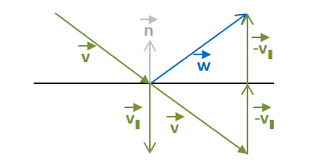
\includegraphics[scale=0.5]{../images/Reflection.png}
\end{center}
The horizontal line in the figure represent a plane $\pi$ while $\underline{n}$ is its normal vector of length 1. 
Given $\underline{v}$ to obtain $\underline{w}$ we can use the following formula:
\[
\underline{w} = \underline{v} - 2(\underline{v}^\intercal \underline{n})\underline{n} = \underbrace{(I - 2\underline{n}\underline{n}^\intercal)}_{\text{reflection matrix}}\underline{v}
\]
Moreover, $R^{-1} = R^\intercal$. This makes sense because if we apply the reflection matrix twice, we obtain the original vector $\underline{v}$, i.e. the reflection of the reflection is the starting vector.

If we didn't have the 2 in the formula, we would obtain the projection of $\underline{v}$ on the plane $\pi$ which is called orthogonal projection and the matrix $R$ would be singular. \\

Let's now dive a bit into the third point of the factorization list. We said that when $S = S^\intercal$ (symmetric matrix) we can factorize it as $S = Q\Lambda Q^\intercal$ where $\Lambda$ is a diagonal matrix and $Q$ is an orthogonal matrix.\\
\[
S = S^\intercal = \underbrace{(Q\Lambda))}_{\tilde{Q}}Q^\intercal = \tilde{Q}Q^\intercal   
\]
\[
\tilde{Q} = \underline{q_1}\underline{\lambda_1} + \dots + \underline{q_n}\underline{\lambda_n}    
\]
Where the $q$ vectors are columns and $\lambda$ vectors are rows. The notation here is a bit confusing but the not matrix $\tilde{Q}$ is not necessarily an orthogonal matrix, only if all eigenvalues of the matrix $\Lambda$ are unitary.
So we can reformulate:
\[
    S = (\underline{q_1}\underline{\lambda_1} + \dots + \underline{q_n}\underline{\lambda_n})Q^\intercal = \underline{q_1}\underline{\lambda_1}\underline{q_1}^\intercal + \dots + \underline{q_n}\underline{\lambda_n}\underline{q_n}^\intercal
\]
This is called \textbf{spectral decomposition} of matrix $S$ and $q_1, \dots, q_n$ are the eigenvectors of $S$ while $\lambda_1, \dots, \lambda_n$ are the eigenvalues of $S$.
\[
    S\underline{q_1} = \lambda_1\underline{q_1} = (\underline{q_1}\underline{\lambda_1}\underline{q_1}^\intercal + \dots + \underline{q_n}\underline{\lambda_n}\underline{q_n}^\intercal)\underline{q_1} = 
    \underline{\lambda_1}\underline{q_1}(\underline{q_1^\intercal}\underline{q_1})
    \]
All the other products are null since the vector $\underline{q_1}$ is orthogonal to all the other vectors $\underline{q_i}$ for $i \neq 1$ (recall that they are eigenvectors).

\section{Null spaces}
Let's consider the starting problem for a linear system of equations:
\[
A\underline{x} = \underline{b} \hspace{1cm} \text{with} \hspace{1cm} A\in \mathbb{R}^{m \times n}, \text{rank($A$)}=r    
\]

We are going to introduce 2 more spaces other than the column ones. To do so we consider:
\[
  A\underline{x} = \underline{0} \hspace{1cm} \rightarrow \hspace{1cm} N(A) \equiv \ker(A) = \{\underline{x} \in \mathbb{R}^n : A\underline{x} = \underline{0}\}  
\]
\[
    A^\intercal\underline{x} = \underline{0} \hspace{1cm} \rightarrow \hspace{1cm} N(A^\intercal) \equiv \ker(A^\intercal) = \{\underline{x} \in \mathbb{R}^n : A^\intercal\underline{x} = \underline{0}\}    
\]

So now, adding the so called \textbf{null spaces} we have that:
\begin{enumerate}
    \item $\mathcal{C}(A) \subset  \mathbb{R}^m$ and $dim(\mathcal{C}(A)) = r$
    \item $\mathcal{C}(A^\intercal) \subset \mathbb{R}^n$ and $dim(\mathcal{C}(A^\intercal)) = r$
    \item $N(A) \subset \mathbb{R}^n$ and $dim(N(A)) = ?$
    \item $N(A^\intercal) \subset \mathbb{R}^m$ and $dim(N(A^\intercal)) = ?$
\end{enumerate}
We still do not know the dimensions of those spaces. 
\subsection*{Null space cardinality}
In the first lecture, we defined 4 spaces: $N(A), N(A^\intercal), \mathcal{C}(A), \mathcal{C}(A^\intercal)$. For the last two we defined also their cardinality whilst for the first ones we weren't able to tell yet. In this lecture we are going to find those values and prove them. In order to do so, we start from few useful properties:
\begin{enumerate}
    \item $\underline{x} = \underline{0} \in N(A)$ for any matrix $A$
    \item if $\underline{x}, \underline{y} \in N(A) \implies A(\underline{x} + \underline{y}) = \underline{0}$
    \item if $\underline{x} \in N(A) \implies \alpha\underline{x}$ with $\alpha \in \mathbb{R} \implies A(\alpha\underline{x}) = \underline{0}$
\end{enumerate}  

Consider, once again, the matrix $A \in \mathbb{R}^{m\times n}$, rank($A$) = $r \leq n$. 
We have seen the decomposition $A = CR$, where $C$ contains the linearly independent columns of $A$ and $R$ contains the coefficients that allow to recover the columns of $A$ starting from its independent columns. 
So, the matrix $A$ can be rewritten as:
\[
  A = \begin{bmatrix}
    A_1 & A_2
  \end{bmatrix} 
  \hspace{1cm}
  A_1 \in \mathbb{R}^{m\times r} \hspace{1cm} A_2 \in \mathbb{R}^{m\times (n-r)} 
\]
Where $A_1$ contains the independent columns of $A$ and $A_2$ the dependent ones.
Example:
\[
A = 
\begin{bmatrix}
    1 & 4 & 7\\
    2 & 5 & 8\\
    3 & 6 & 9
\end{bmatrix}
= 
\underbrace{
\begin{bmatrix}
1 & 4\\
2 & 5\\
3 & 6
\end{bmatrix}}_{A_1}
\begin{bmatrix}
    1 & 0 & -1\\
    0 & 1 & \undermat{B}{2}
\end{bmatrix}
\]
Since we have the last column of $A$, that is linearly dependent so it belongs to $A_2$, we can reformulate it in this way:
\[
    A = \begin{bmatrix}
        A_1 & A_2
      \end{bmatrix} 
    = \begin{bmatrix}
        A_1 & A_1B
    \end{bmatrix}
\]
We build a new matrix $K$ defined as follows:
\[
    K = \begin{bmatrix}
        -B\\
        I_{n-r}
    \end{bmatrix}
    \hspace{1cm}
    K \in \mathbb{R}^{n\times(n-r)}    
    \hspace{1cm}
    B \in \mathbb{R}^{r\times(n-r)}    
\]

\[
AK = \begin{bmatrix}
    A_1 & A_1B
\end{bmatrix} 
\begin{bmatrix}
    -B\\
    I_{n-r}
\end{bmatrix}
= A_1(-B) + A_1B = 0   
\]
Where the last 0 is actually a matrix of zeros of dimension $m\times(n-r)$
because A has size $m\times n$ and $K$ has size $n\times(n-r)$.
We have that:
\[
    AK = 0 \implies A\underline{k_i} = 0 \hspace{1cm} \forall i \in \{1, \dots, n-r\}    
\]
Where $k_i$ is the i-th column of $K$. This means that: $\underline{k_i} \in N(A) \hspace{0.2cm} \forall i$.

Now, we want to demonstrate that: $K\underline{u} = 0 \implies \underline{u} = \underline{0}$. 
To do so, we start from expanding $K$ from its definition:
\[
    K = \begin{bmatrix}
        -B\\
        I
    \end{bmatrix}
    \underline{u} = 0
    \implies
    \begin{bmatrix}
        -B\underline{u}\\
        \underline{u}
    \end{bmatrix}
    = 
    \begin{bmatrix}
        \underline{0}\\
        \underline{0}
    \end{bmatrix}
\]
Where the two zero vectors have dimension $r$ and $n-r$ respectively! Considering the second row of the matrix we get: $\underline{u} = \underline{0}$ so all columns of $K$ are linearly independent.\\

If we consider the problem ($\star$) $A\underline{x} = \underline{0}$, we want to prove that each \underline{x} that satisfy ($\star$) must be a linear combination of the columns of $K$.\\
\[
    A_1\underline{x} = \underline{0} \in \mathbb{R}^m \implies \underline{x} = \underline{0} \in \mathbb{R}^r    
\]
Because $A_1$ has linearly independent columns, i.e. has full rank.
\[
    A\underline{u} = \underline{0} \in \mathbb{R}^m \implies \begin{bmatrix}
        A_1 & A_1B
    \end{bmatrix} 
    \begin{bmatrix}
        \underline{u_1}\\
        \underline{u_2}
    \end{bmatrix}  
    = 
    \begin{bmatrix}
        A_1\underline{u_1} + A_1B\underline{u_2}\\
    \end{bmatrix}
    = 
    A_1\left[\underline{u_1} + B\underline{u_2}\right]
    = \underline{0}
\]
We can notice that the last formulation obtained in the equation has the same form as the one from where we started the proof, so we can say that:
\[
    \underline{u_1} + B\underline{u_2} = \underline{0} \implies \underline{u_1} = -B\underline{u_2}    
\]
\[
   \underline{u} = \begin{bmatrix}
    -B\underline{u_2}\\
    \underline{u_2}
\end{bmatrix}
    =
\underbrace{\begin{bmatrix}
    -B\\
    I
\end{bmatrix}}_{K}
    \underline{u_2}
    = K\underline{u_2}
    \implies 
    dim(N(A)) = n - r
\]


\begin{center}
    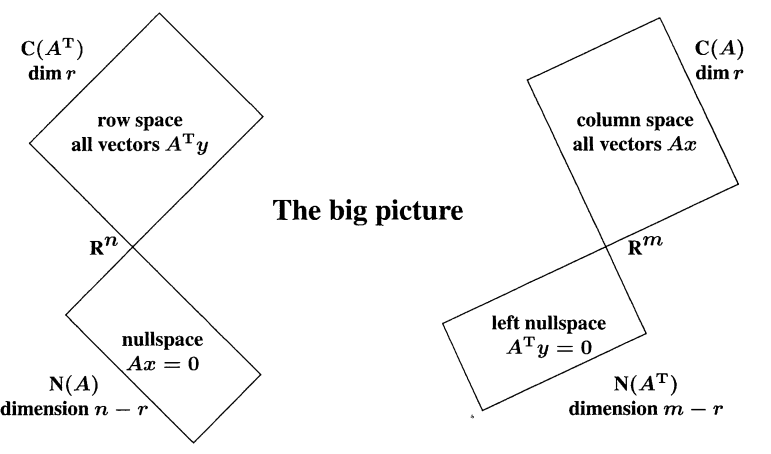
\includegraphics[scale = 0.4]{../images/SpacesDimensions.png}
\end{center}


\\



